\chapter{Лабораторная работа №8. Программирование синтезатора частот с управлением по IIC}

\section{Интерфейс IIC}

Шина IIC содержит линию данных (SDA) и линию тактового сигнала (SCL). 
Каждое устройство распознается по уникальному адресу.
Кроме того, устройства могут быть классифицированы как ведущие и ведомые при передаче данных.
Ведущий - это устройство, которое инициирует передачу данных и
вырабатывает тактовый сигнал. При этом любое адресуемое устройство считается
ведомым по отношению к ведущему. 

Шина IIC допускает несколько ведущих. Это означает, что более чем одно устройство, 
способное управлять шиной, может быть подключено к ней.
Возможность подключения более одного микроконтроллера к шине означает, что более
чем один ведущий может попытаться начать пересылку в один и тот же момент времени. 
Для устранения хаоса, который может возникнуть в данном случае, разработана
процедура арбитража. Эта процедура основана на том, что все IIC - устройства подключаются к шине по правилу монтажного И.

Данные на линии SDA должны быть стабильными в течение ВЫСОКОГО периода
синхроимпульса. ВЫСОКОЕ или НИЗКОЕ состояние линии данных должно меняться, 
только если линия синхронизации в состоянии НИЗКОЕ (см. Рисунок 3). 

Как SDA, так и SCL являются двунаправленными линиями, подсоединенными к
положительному источнику питания через подтягивающий резистор (см. Рисунок 2). 
Когда шина свободна, обе линии находятся в ВЫСОКОМ положении. Выходные каскады
устройств, подключенных к шине, должны иметь открытый сток или открытый коллектор
для обеспечения функции монтажного И. Данные по шине I2
C могут передаваться со скоростю до 100 кбит/с в стандартном режиме, и до 400 кбит/с в "быстром" режиме. 

Специальные ситуации на шине отмечают сигналы START и STOP (см. Рисунок 4). 
Переход линии SDA из ВЫСОКОГО состояния в НИЗКОЕ, в то время как SCL находится
в ВЫСОКОМ состоянии означает START. 
Переход линии SDA из НИЗКОГО состояния в ВЫСОКОЕ при SCL в ВЫСОКОМ
состоянии означает STOP. 
Сигналы СТАРТ и СТОП всегда вырабатываются ведущим. Считается, что шина занята
после сигнала СТАРТ. Шина считается освободившейся через определенное время после
сигнала СТОП. 

Каждый байт, передаваемый по линии SDA, должен состоять из 8 бит. Количество байт, передаваемых за один сеанс связи неограничено. Каждый байт должен оканчиваться битом подтверждения. Данные передаются, начиная с наиболее значащего бита (см. Рисунок 5). Если приёмник не может принять еще один целый байт, пока он не выполнит какую-либо другую функцию (например, обслужит внутреннее прерывание), он может удерживать линию SCL в НИЗКОМ состоянии, переводя передатчик в состояние ожидания. Пересылка данных продолжается, когда приёмник будет готов к следующему байту и отпустит линию SCL.

Подтверждение при передаче данных обязательно. Соответствующий испульс
синхронизации генерируется ведущим. Передатчик отпускает (ВЫСОКОЕ) линию SDA в
течение синхроимпульса подтверждения. Приёмник должен удерживать линию SDA в
течение ВЫСОКОГО состояния синхроимпульса подтверждения в стабильно НИЗКОМ
состоянии (Рисунок 6). Конечно, время установки и удержания также должны быть
приняты во внимание (см. Раздел 13.0 Электрические и временные параметры).

\section{Организация шины IIC на плате VC707}

На отладочной плате VC707 к FPGA подключен только один интерфейс IIC, 
который подлючается к 8 устройствам через мультиплексор шины IIC - PCA9548.
Коммутатор шины может работать на скоростях до 400 кГц. Адрес I2C коммутатора шины — 0x74 (0b1110100), 
его необходимо адресовать и настроить для выбора нужного коммутируемого устройства.

\begin{figure}[h]
	\centering
	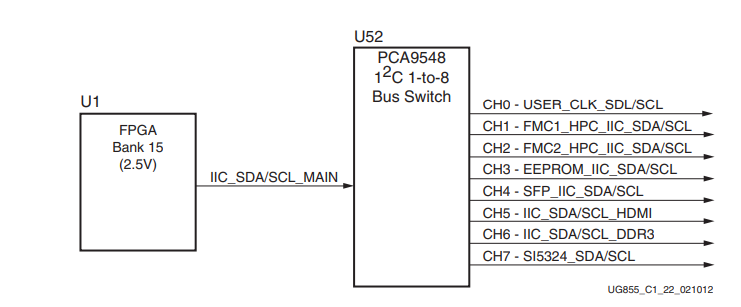
\includegraphics[width=0.6\textwidth]{image/PCA9548.png}
	\caption{Вкладка "AXI4-Stream Options"}
	\label{PCA9548.PNG}
\end{figure}

\begin{table}[!ht]
	\begin{center}
		\begin{tabular}{c c c c c}
			\hline\hline
			Устройство & Номер порта коммутатора &  IIC адрес \\
			\hline
			PCA9548 		& NA &	0b1110100  \\
			Si570 Clock 	& 0 & 	0b1011101  \\
			FMC1 HPC 		& 1 & 	0bXXXXX00  \\
			FMC2 HPC 		& 2 & 	0bXXXXX00  \\
			M24C08 EEPROM 	& 3 & 	0b1010100   \\
			SFP Модуль 		& 4 & 	0b1010000   \\
			ADV7512 HDMI 	& 5 & 	0b0111001  \\
			DDR3 SODIMM 	& 6 & 	0b1010000, 0b0011000  \\
			Si5324 Clock 	& 7 & 	0b1101000  \\
			\hline
		\end{tabular}
		\caption{Подключение индикатора к ПЛИС}
		\label{LCD_TO_FPGA}
	\end{center}
\end{table}

По условию START мастер шины должен вывести адрес ведомого, к которому он обращается. Адрес PCA9548 показан на рис. 3. Для экономии энергии на аппаратно выбираемых контактах адреса нет внутренних подтягивающих резисторов, и они должны быть подтянуты к ВЫСОКОМУ или НИЗКОМУ уровню.Последний бит адреса ведомого определяет операцию, которая будет выполненный. При установке на логическую 1 выбирается чтение, а на логический 0.
выбирает операцию записи.

\begin{figure}[h]
	\centering
	
\includegraphics[width=0.5\textwidth]{image/PCA9548_addr.png}
	\caption{Вкладка "AXI4-Stream Options"}
	\label{PCA9548_addr.PNG}
\end{figure}

\begin{figure}[h]
	\centering
	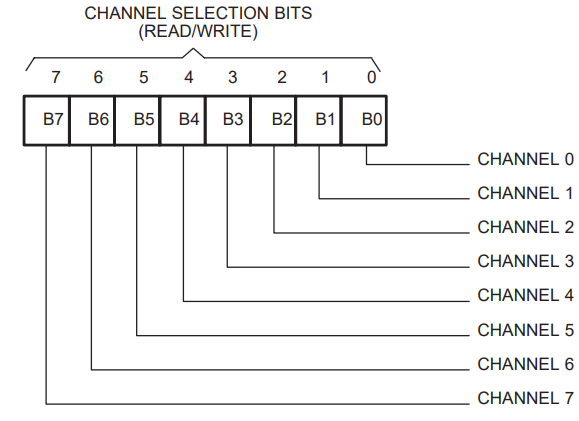
\includegraphics[width=0.5\textwidth]{image/PCA9548_CR.png}
	\caption{Вкладка "AXI4-Stream Options"}
	\label{PCA9548_CR.PNG}
\end{figure}

После успешного подтверждения адреса ведомого,
мастер шины отправит байт на PCA9548, который будет сохранен
в регистре управления. Если несколько байтов получены
PCA9548 сохранит последний полученный байт. Этот регистр может быть
записывается и читается по шине I2C.
Одна или несколько нисходящих пар или каналов SCx/SDx выбираются по содержимому управляющего регистра. Этот регистр записывается после обращения к PCA9548. 2 младших бита управляющего байта используются для определения того, какой канал следует выбрать. Когда канал выбран, он становится активным после того, как на шине I2C будет установлено условие остановки. Это гарантирует, что все линии SCx/SDx будут находиться в состоянии HIGH, когда канал станет активным, так что во время соединения не будут генерироваться ложные условия.

Вход RESET представляет собой активный НИЗКИЙ сигнал, который можно использовать для восстановления после неисправности шины. Установив этот сигнал НИЗКИМ в течение как минимум tWL, PCA9548 сбросит свои регистры и конечный автомат I2C и отменит выбор всех каналов. Вход RESET должен быть подключен к VDD через подтягивающий резистор.
Когда на VDD подается питание, внутренний сброс при включении питания удерживает PCA9548 в состоянии сброса до тех пор, пока VDD не достигнет VPOR. В этот момент условие сброса отменяется, и регистры PCA9548 и конечный автомат I2C инициализируются до своих состояний по умолчанию, все нули вызывают отмену выбора всех каналов.

\section{Синтезатор частот Si570}

\begin{figure}[h]
	\centering
	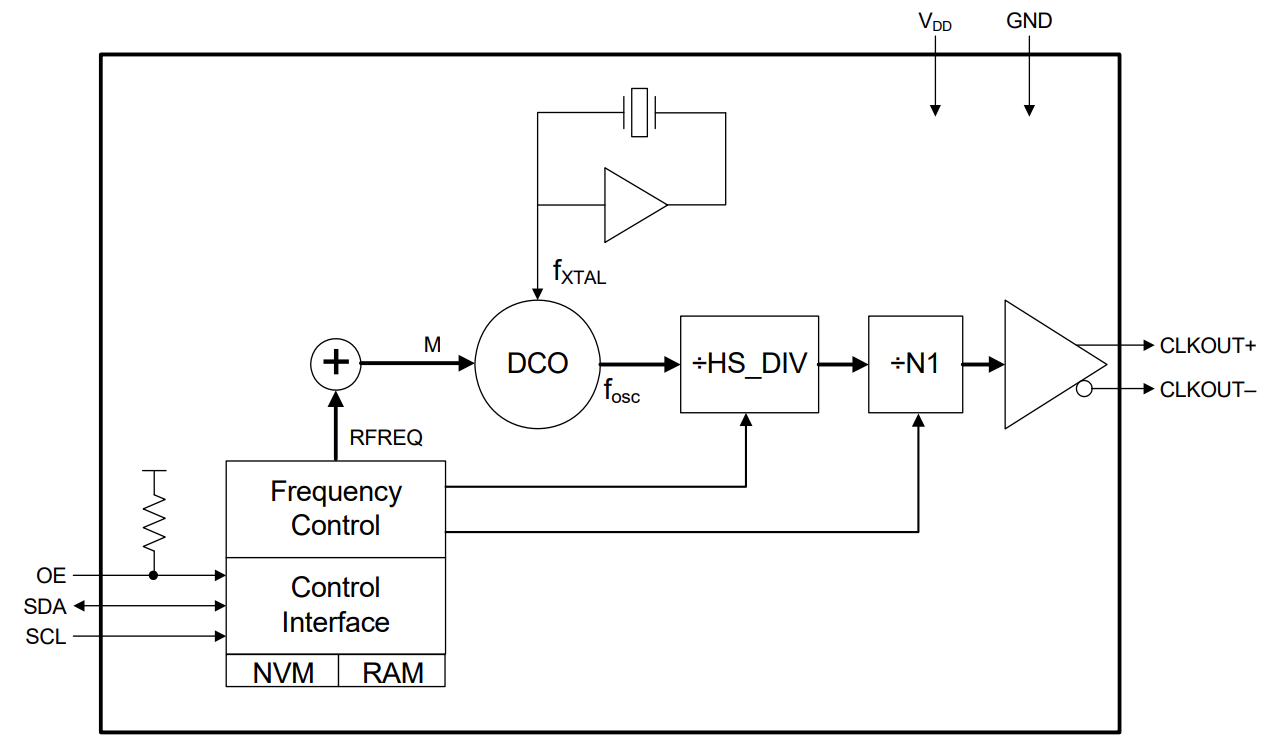
\includegraphics[width=0.5\textwidth]{image/Si570.png}
	\caption{Структурная схема синтезатора частот Si570}
	\label{Si570.PNG}
\end{figure}

\subsection{Программирование новой выходной частоты}

Выходная частота \(F_{OUT}\) определяется путем программирования частоты генератора c цифровым управлением \(F_{DCO}\) и выходных делителей устройства (\(HS\_DIV\), N1) и рассчитывается по следующему уравнению:

\begin{equation}	
	F_{OUT} = \frac{F_{XTAL} \cdot RFREQ}{HS\_DIV \cdot N1}.
\end{equation}

Частота \(F_{DCO}\) регулируется в диапазоне от 4,85 до 5,67 ГГц путем установки 38-битного дробного множителя высокого разрешения \(RFREQ\). Частота \(F_{DCO}\) является произведением частоты (\(F_{XTAL}\)) внутреннего кварцевого резонатора и \(RFREQ\). 38-битное разрешение RFREQ позволяет частоте \(F_{DCO}\) иметь программируемое разрешение по частоте 0,09 ppb.

\begin{figure}[h]
	\centering
	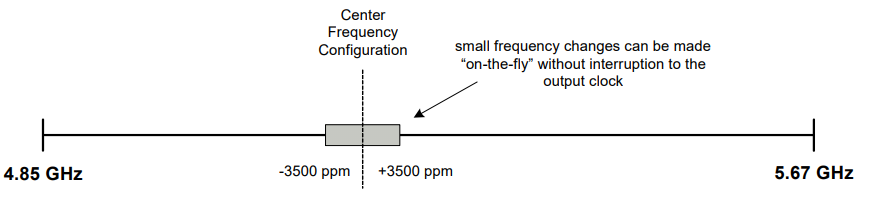
\includegraphics[width=0.5\textwidth]{image/si570_0.png}
	\caption{Структурная схема синтезатора частот Si570}
	\label{si570_0.PNG}
\end{figure}

Как показано на рис.~\ref{si570_0.PNG}, устройство позволяет перепрограммировать частоту \(F_{DCO}\) в диапазоне ±3500 относительно центральной частоты без прерывания формирования выходной тактовой частоты. Изменения частоты, выходящие за пределы окна ±3500, приведут к перекалибровке внутренней схемы интервалов времени, в результате чего формирование выходной частоты моментально остановится, и запустится в произвольной точке периода тактов. Этот процесс перекалибровки установит новую центральную частоту, что займет по времени до 10 мс. Схемы, получающие тактирование от устройства Si570, чувствительные к выбросам (искажениям) тактового сигнала, может понадобиться сбросить после того, как завершится процесс перекалибровки Si570.

Когда выходную частоту нужно поменять на большее значение, чем окно ±3500 ppm от центральной частоты, то потребуется перепрограммировать как частоту DCO, так и выходные делители. Имейте в виду, что такое изменение частоты DCO за пределами окна ±3500 ppm приведет к тому, что выдача выходного сигнала тактов моментально остановится, и запустится в произвольной точке периода тактов. Поэтому для чувствительных устройств, получающих такое прерывистое тактирование (например процессоры, MCU) может понадобиться сброс после того, как завершилась перестройка частоты Si57x.

\textbf{Пример}: Si570, генерирующий 156,25 МГц, должен быть переконфигурирован на частоту 161,1328125 МГц (156,25 MHz x 66/64). Это изменение частоты больше, чем ±3500 ppm. Алгоритм программирования Si570 состоит из следующих этапов:

\begin{enumerate}
	\item Прочитайте из устройства конфигурацию первоначальной частоты запуска (RFREQ, HSDIV и N1), которая устанавливается после включения питания или сброса. Значения регистров текущей конфигурации: 7 - 0x01, 8 - 0xC2, 9 - 0xBC, 10 - 0x01,
	11 - 0x1E, 12 - 0xB8. Из значений регистров получаем следующие переменные:

	\begin{equation}	
		RFREQ = 2BC011EB8h / 228 = 43,75027344;
	\end{equation}
	
	\begin{equation}	
		HSDIV = 0x0 = 4;
	\end{equation}
	
	\begin{equation}	
		N1    = 0x7 = 8.
	\end{equation}

	\item Из-за незначительных вариаций частоты внутреннего кварца от одной микросхемы Si570 к другой каждая микросхема может иметь отличающееся значение RFREQ, или даже могут быть разные значения HSDIV или N1 для одной и той же выходной частоты. По этой причине требуется вычисление \(F_{XTAL}\) для каждого устройства. Вычисление действительной номинальной частоты кварцевого резонатора производим по формуле:

	\begin{equation}	
		F_{XTAL} = \frac{F_{0} \cdot HSDIV \cdot N1}{RFREQ} = 114,285000000 МГц,
	\end{equation}

	где \(F_{0}\) - выходная частота первоначального запуска.

	\item Выберите новую выходную частоту \(F_{1}\):

	\begin{equation}	
		F_{1} = 161,132812000 МГц.
	\end{equation}

	\item Первый шаг ручного вычисления конфигурации частоты состоит в определении новых значений делителя частоты (HSDIV, N1). По значению нужной выходной частоты находят такие коэффициенты деления делителя, которые сохраняют частоту DCO в диапазоне 4.85 .. 5.67 ГГц. Для HSDIV допустимы значения 4, 5, 6, 7, 9 или 11. Значение N1 может быть выбрано равное 1 или любому четному числу до 128 включительно (т. е. 1, 2, 4, 6, 8, 10, .., 128). Чтобы помочь в минимизации энергопотребления, должны быть выбраны значения коэффициентов деления таким образом, чтобы частота генерации DCO была как можно меньше. Самое маленькое значение N1 с самым большим значением HSDIV также приведет к самому низкому потреблению энергии.

	\begin{equation}	
		F_{DCO\_NEW} =  \frac{F_{OUT\_NEW} \cdot HSDIV_{NEW} \cdot N1_{NEW}}{RFREQ} = 5,156249984 ГГц,
	\end{equation}

	\begin{equation}	
		HSDIV = 0x0 = 4,
	\end{equation}
	
	\begin{equation}	
		N1 = 0x7 = 8.
	\end{equation}
	
	\item Как только HSDIV и N1 определены, следующий шаг - вычисление коэффициента умножения опорной частоты (RFREQ). Вычислите новый коэффициент умножения частоты кварца \(RFREQ\) по формуле:

	\begin{equation}	
		RFREQ = \frac{F_{DCO}}{F_{XTAL}} = 45,11746934;
	\end{equation}

	\begin{equation}	
		45,11746934 \cdot 228 = 2D1E12788h.
	\end{equation}

	RFREQ программируется как 38-разрядное дробное число множителя частоты, где первые 10 самых старших бит (MSB) представляют целую часть этого множителя, и 28 младших значащих бит (LSB) представляют дробную часть.

	Перед тем, как вводить дробную часть в регистр RFREQ, она должна быть преобразована в 38-разрядное целое число битовой операцией сдвига влево на 28 бит, что эффективно умножит RFREQ на 228.

	Рассмотрим пример. Пусть 
	
	\begin{equation}	
		RFREQ =  46,043042064,
	\end{equation}

	тогда умножим RFREQ на 228, получаем

	\begin{equation}	
		RFREQ \cdot 228 =  12359584992,1,
	\end{equation}

	отбросим дробную часть, получаем 

	\begin{equation}	
		RFREQ =  12359584992,
	\end{equation}

	теперь преобразуем в шестнадцатеричное значение, получаем

	\begin{equation}	
		RFREQ = 02E0B04CE0h.
	\end{equation}

	В примере выше операция умножения требует 38-битной точности. Если такая 38-разрядная арифметика недоступна, то дробную часть можно отделить от целой, и сдвинуть влево на 28 бит. Результат склеивается с целой частью для формирования полного 38-битного слова. Пример этой операции показан на рис. 4.

	\item Остановите DCO установкой Freeze DCO = 1 (бит 4 регистра 137).

	\item Запишите новую конфигурацию частоты (\(RFREQ\), \(HSDIV\), and \(N1\)). Значение регистров новой конфигурации: 
	7 - 0x01, 8 - 0xC2, 9 - 0xD1, 10 - 0xE1, 11 - 0x27, 12 - 0x88.
	\item Разрешите работу DCO установкой Freeze DCO = 0 и выставите бит NewFreq (бит 6 регистра 135) на 10 мс.
\end{enumerate}

\subsection{Перенастройка выходной частоты в малом диапазоне}

Для изменений выходной частоты в пределах ±3500 ppm относительно центральной требуется перепрограммировать 
только частоту \(F_{DCO}\). Поскольку \(F_{DCO}\) = \(F_{XTAL} \cdot RFREQ\) и частота \(F_{XTAL}\) фиксирована, то частота \(F_{DCO}\) переконфигурируется простым изменением коэффициента RFREQ по процедуре, описанной ниже:

\begin{enumerate}
	\item Через IIC считывается текущее значение \(RFREQ\) (адреса 7..12 для всех устройств Si571 и Si570 с термостабильностью 20 ppm и 50 ppm; или адреса 13..18 для устройств Si570 с термостабильностью 7 ppm).

	\item Вычисляется новое значение \(RFREQ\) в соответствии с изменением частоты:
	
	\begin{equation}	
		RFREQ_{NEW} =  RFREQ_{CURRENT} \cdot \frac{F_{OUT\_NEW}}{F_{OUT\_CURRENT}},
	\end{equation}

	\item Через IIC записывается новое значение \(RFREQ\) (по тем же адресам, по которым это значение было прочитано на шаге 1).
\end{enumerate}

\textbf{Пример}: Si570 генерирует частоту 148.35 МГц, которую нужно перестроить "на лету" для генерации 148.5 МГц. Это изменение составит +1011.122 ppm, что укладывается в окно ±3500 ppm.

Типовая конфигурация для этого примера:

\begin{equation}	
	RFREQ_{CURRENT} =  2EBB04CE0h,
\end{equation}

\begin{equation}	
	F_{OUT\_CURRENT} =  148.35 МГц,
\end{equation}

\begin{equation}	
	F_{OUT\_NEW} = 148.50 МГц.
\end{equation}

Вычисляем новое значение \(RFREQ\) для изменения выходной частоты от 148,35 МГц к 148,5 МГц:

\begin{equation}	
	RFREQ_{NEW} = 2EC71D666h,
\end{equation}

\textbf{Замечание}: вычислительные операции над \(RFREQ\) потребуют как минимум 38-разрядной арифметической точности.

Даже относительно небольшие изменения выходной частоты могут потребовать записи больше одного регистра \(RFREQ\). Поэтому такая многорегистровая запись может отрицательно сказаться на выходной частоте, пока эти регистры обновляются по очереди.

Предотвратить эти временные колебания выходной тактовой частоты во время записи регистров \(RFREQ\) можно следующей процедурой:

\begin{enumerate}
	\item Заморозка значения "M" (установка в 1 бита 5 регистра 135). 
	\item Запись новой конфигурации частоты (регистров \(RFREQ\)).
 	\item Разморозка значения "M" (установка в 0 бита 5 регистра 135).
\end{enumerate}

\section{AXI IIC Bus Interface IP Core}
\begin{figure}[!ht]
	\centering
	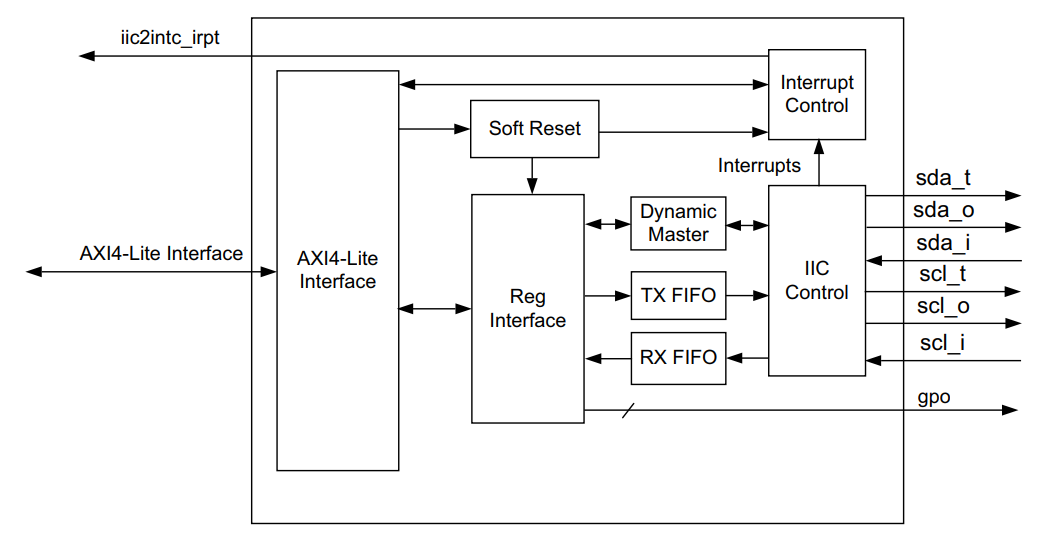
\includegraphics[width=0.5\textwidth]{image/IIC_core_0.png}
	\caption{Структурная схема AXI IIC Bus Interface IP Core}
	\label{IIC_core_0.PNG}
\end{figure}


\section{Проект в Vivado}

\section{Проект в Xilinx SDK}